% Тезис
% Аргумент
% Пример

{\actuality} 
% Тезис
Повседневную деятельность человека на текущем этапе 
технологического развития невозможно представить без автоматизации, 
использования роботизированных механизмов, информационных сервисов и 
вычислительных сетей. 
% Аргумент
Их повсеместное использование позволяет значительно повышать производительность 
труда, а так же решать невыполнимые или трудновыполнимые ранее задачи.
% Пример
Так, согласно отчету компании Ipsos и Всемирного экономического форума 
<<Global citizens \& Automation>> за 2019 год, около 46\% работников во всем 
мире считают, что благодаря автоматизации их работа кардинально изменилась за 
прошедшие 10 лет, и склонны положительно оценивать изменения, которые она принесла.

% Тезис
Особенное заметны изменения, связанные с применением мобильных интернет-сетей, 
дронов (беспилотных летательных аппаратов, БПЛА) и роботизированных механизмов. 
% Аргумент
%TODO: написать сферы применимости дронов и мобильных сетей
% Пример
%TODO: сделать ссылки на исследования проникновения дронов и мобильных сетей
% https://www.mdpi.com/journal/drones/special_issues/5663HCFN3X

Настоящее исследование посвящено технологиям привязных дронов --- 
высотных телекоммуникационных платформ (ВТП). %TODO: Ссылки на обзорные материалы по привязным платформам
%TODO: сделать небольшой обзор сфер применимости привязных платформ
В частности, рассматривается проблема методов навигации ВПТ во время полета с 
полезной нагрузкой и во время взлёта/посадки на стартовую площадку. 
% Тезис
Технология определения дроном своего местоположения в пространстве критически 
необходима для его работы. 
% Аргумент
Для реальной системы невозможно ее корректное перемещение без получения обратной
связи по изменению положения в ответ на усилие двигательных и рулевых элементов.
% Пример
Для беспилотных систем, управляемых оператором, такой обратной связью может 
выступать визуальное наблюдение самой системы или информация с видеокамеры и 
других датчиков, размещенных на аппарате.
    % Вложенный тезис
    Однако для систем с автоматическим управлением интерпретация таких данных 
    --- непростая задача. 
    % Вложенный аргумент
    Бортовой компьютер может воспринимать и обрабатывать 
    лишь числовые данные с датчиков и алгоритмов.
    % Вложенный пример
    Например, такие данные предоставляют:
    \begin{enumerate}
        \item датчики систем спутниковой навигации (GNSS): 
        % \begin{enumerate}
        %     \item GPS, 
        %     \item ГЛОНАСС,
        %     \item Galileo, 
        %     \item Baidu. 
        % \end{enumerate} 
        \item Датчики высоты (напр. барометрические)
        \item Системы радиолокации
        \item Системы на основе обработки видео
        \item Системы на основе дальнометров и лидаров
        \item Системы на основе акселерометров и гироскопов
    \end{enumerate} 
    При этом такие методы навигации можно условно разделить на глобальные 
    (спутниковая навигация, дальняя радиолокация) и локальные 
    (в пределах локальной области использования платформы).

% Тезис
Разработка методов локальной навигации представляет особый научный и практический 
интерес.
% Аргумент
Сервисы спутниковой навигации представляют ограниченную точность, %TODO: уточнить значение
могут не иметь покрытия в определенных условиях и могут конкурировать за 
радиочастотные ресурсы с другими системами и сервисами.
% Пример

В этой работе исследуется один из методов локальной навигации: 
с помощью технологии считывания RFID и барометрического датчика высоты. 
Общая схема предлагаемой системы навигации представлена на рисунке: %TODO: вставить рисунок
\begin{figure}[ht]
    \begin{center}
        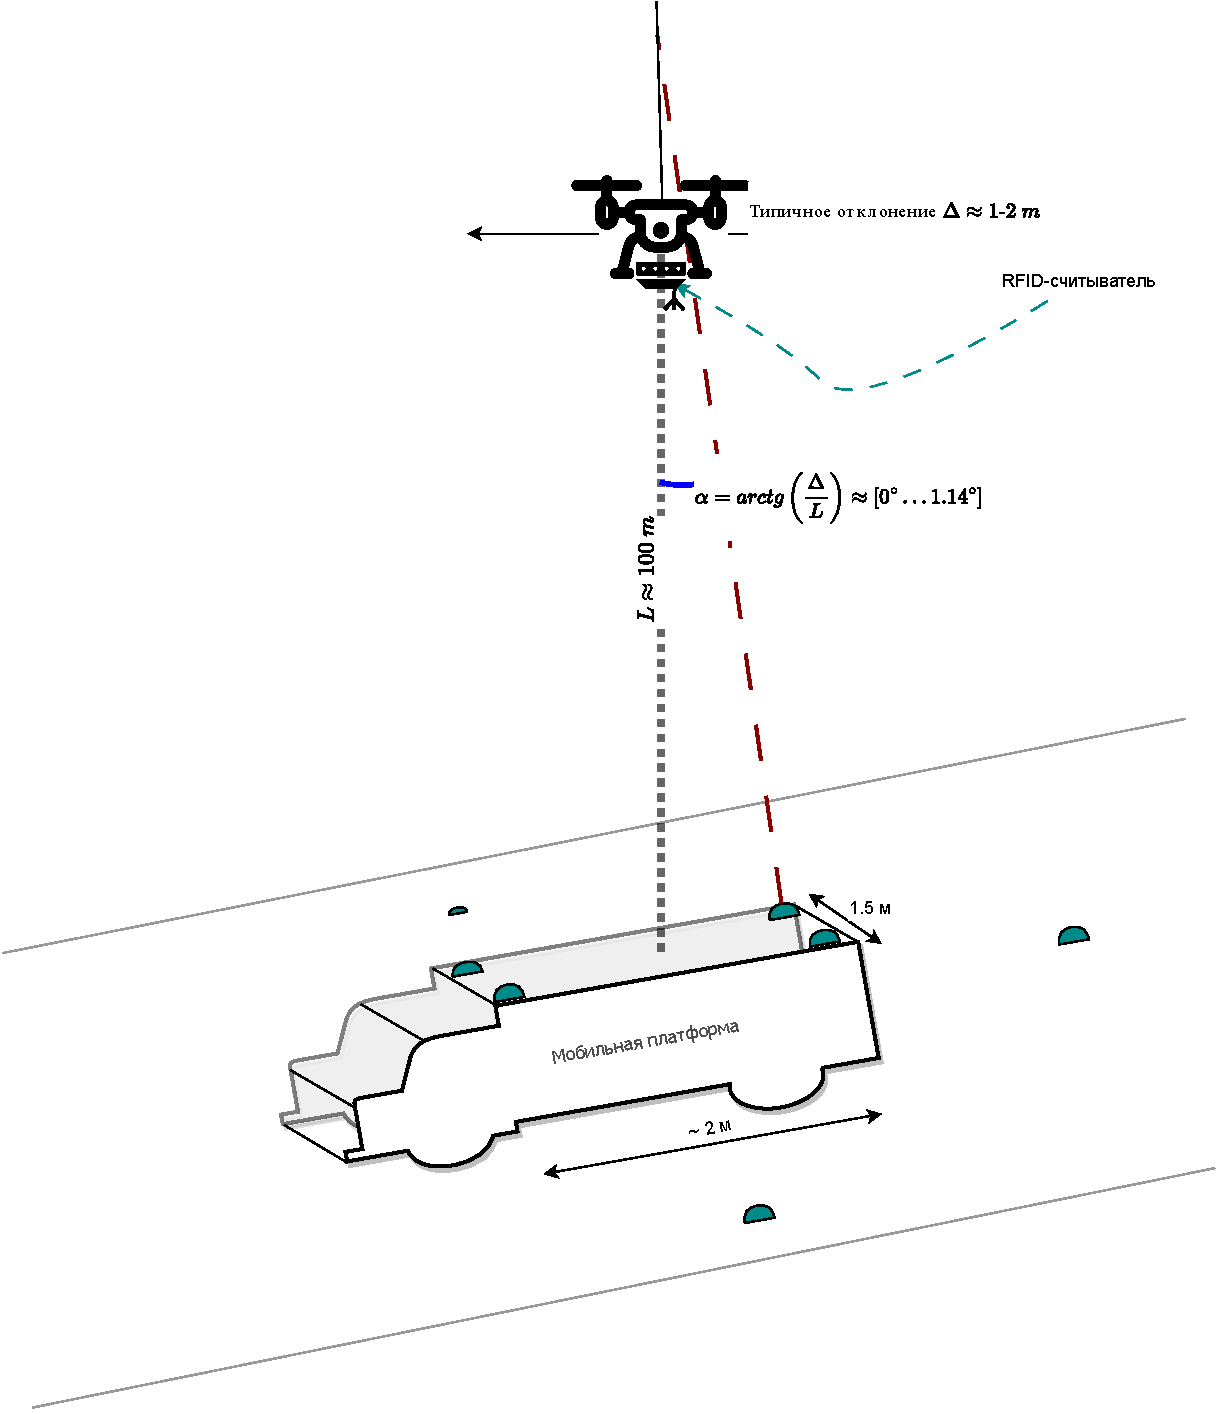
\includegraphics[width=0.85\linewidth]{Dissertation/images/rfid_navigation_general_schema.pdf}
        \caption{Общая схема исследуемой системы}\label{fig:intro_gen_schema}
    \end{center}
\end{figure}
% Тезис
% Аргумент
% Пример

% Обзор, введение в тему, обозначение места данной работы в
% мировых исследованиях и~т.\:п., можно использовать ссылки на~другие
% работы~\autocite{Gosele1999161,Lermontov}
% (если их~нет, то~в~автореферате
% автоматически пропадёт раздел <<Список литературы>>). Внимание! Ссылки
% на~другие работы в~разделе общей характеристики работы можно
% использовать только при использовании \verb!biblatex! (из-за технических
% ограничений \verb!bibtex8!. Это связано с тем, что одна
% и~та~же~характеристика используются и~в~тексте диссертации, и в
% автореферате. В~последнем, согласно ГОСТ, должен присутствовать список
% работ автора по~теме диссертации, а~\verb!bibtex8! не~умеет выводить в~одном
% файле два списка литературы).
% При использовании \verb!biblatex! возможно использование исключительно
% в~автореферате подстрочных ссылок
% для других работ командой \verb!\autocite!, а~также цитирование
% собственных работ командой \verb!\cite!. Для этого в~файле
% \verb!common/setup.tex! необходимо присвоить положительное значение
% счётчику \verb!\setcounter{usefootcite}{1}!.

% Для генерации содержимого титульного листа автореферата, диссертации
% и~презентации используются данные из файла \verb!common/data.tex!. Если,
% например, вы меняете название диссертации, то оно автоматически
% появится в~итоговых файлах после очередного запуска \LaTeX. Согласно
% ГОСТ 7.0.11-2011 <<5.1.1 Титульный лист является первой страницей
% диссертации, служит источником информации, необходимой для обработки и
% поиска документа>>. Наличие логотипа организации на~титульном листе
% упрощает обработку и~поиск, для этого разметите логотип вашей
% организации в папке images в~формате PDF (лучше найти его в векторном
% варианте, чтобы он хорошо смотрелся при печати) под именем
% \verb!logo.pdf!. Настроить размер изображения с логотипом можно
% в~соответствующих местах файлов \verb!title.tex!  отдельно для
% диссертации и автореферата. Если вам логотип не~нужен, то просто
% удалите файл с~логотипом.

% \ifsynopsis
% Этот абзац появляется только в~автореферате.
% Для формирования блоков, которые будут обрабатываться только в~автореферате,
% заведена проверка условия \verb!\!\verb!ifsynopsis!.
% Значение условия задаётся в~основном файле документа (\verb!synopsis.tex! для
% автореферата).
% \else
% Этот абзац появляется только в~диссертации.
% Через проверку условия \verb!\!\verb!ifsynopsis!, задаваемого в~основном файле
% документа (\verb!dissertation.tex! для диссертации), можно сделать новую
% команду, обеспечивающую появление цитаты в~диссертации, но~не~в~автореферате.
% \fi

% {\progress}
% Этот раздел должен быть отдельным структурным элементом по
% ГОСТ, но он, как правило, включается в описание актуальности
% темы. Нужен он отдельным структурынм элемементом или нет ---
% смотрите другие диссертации вашего совета, скорее всего не нужен.

{\aim} данной работы является 
разработка системы локального позиционирования на основе технологии UHF RFID для
управления полетом высотной привязной платформы.% в условиях искажений сигналов GPS/ГЛОНАСС.

Для~достижения поставленной цели необходимо было решить следующие {\tasks}:
\begin{enumerate}[beginpenalty=10000] % https://tex.stackexchange.com/a/476052/104425
    \item Обзор технических методов и литературы в области исследования:
    \begin{enumerate}
        \item Изучить и составить обзор существующих методов локальной навигации 
              беспилотных систем и летательных аппаратов.
        \item Изучить и составить обзор по применимости технологий радиочастотной
              идентификации на БПЛА, транспортных средствах, других подвижных сетях.
        \item Исследовать и изучить стандарты и принципы функционирования.
              технологии RFID.
    \end{enumerate}
    \item Теоретическая часть:
    \begin{enumerate}
        \item Разработать облик системы по расчету положения ВТП на основе 
              информации о считывании RFID-меток и данных с барометрического датчика.
        \item Построить математическую модель взаимодействия считывателя и меток.
        \item Оценить точность, скорость обработки контрольных взаимодействий 
              при различных пространственных конфигурациях элементов системы.
        \item Рассчитать энергетическое потребление элементов системы, сложность 
              настройки и установки, общую стоимость в сравнении с другими 
              методами локальной навигации.
    \end{enumerate}
    \item Практическая часть:
    \begin{enumerate}
        \item Изучить доступные варианты оборудования для реализации системы.
        \item Разработать схему взаимодействия и обработки контрольной информации
              для передачи в интерфейс локальной навигации полетного контроллера.
        \item Разработать программный код обработчика данных, получаемых считывателем.
        % \item Реализовать экспериментальный образец для испытаний на разрабатываемой
        %       в лаб. 69 ИПУ высотной привязной платформе.     
    \end{enumerate}    
\end{enumerate}


{\novelty}
\begin{enumerate}[beginpenalty=10000] % https://tex.stackexchange.com/a/476052/104425
  \item Впервые \ldots
  \item Впервые \ldots
  \item Было выполнено оригинальное исследование \ldots
\end{enumerate}

{\influence} \ldots

{\methods} \ldots

{\defpositions}
\begin{enumerate}[beginpenalty=10000] % https://tex.stackexchange.com/a/476052/104425
  \item Первое положение
  \item Второе положение
  \item Третье положение
  \item Четвертое положение
\end{enumerate}
В папке Documents можно ознакомиться с решением совета из Томского~ГУ
(в~файле \verb+Def_positions.pdf+), где обоснованно даются рекомендации
по~формулировкам защищаемых положений.

{\reliability} полученных результатов обеспечивается \ldots \ Результаты находятся в соответствии с результатами, полученными другими авторами.


{\probation}
Основные результаты работы докладывались~на:
перечисление основных конференций, симпозиумов и~т.\:п.

{\contribution} Автор принимал активное участие \ldots

\ifnumequal{\value{bibliosel}}{0}
{%%% Встроенная реализация с загрузкой файла через движок bibtex8. (При желании, внутри можно использовать обычные ссылки, наподобие `\cite{vakbib1,vakbib2}`).
    {\publications} Основные результаты по теме диссертации изложены
    в~XX~печатных изданиях,
    X из которых изданы в журналах, рекомендованных ВАК,
    X "--- в тезисах докладов.
}%
{%%% Реализация пакетом biblatex через движок biber
    \begin{refsection}[bl-author, bl-registered]
        % Это refsection=1.
        % Процитированные здесь работы:
        %  * подсчитываются, для автоматического составления фразы "Основные результаты ..."
        %  * попадают в авторскую библиографию, при usefootcite==0 и стиле `\insertbiblioauthor` или `\insertbiblioauthorgrouped`
        %  * нумеруются там в зависимости от порядка команд `\printbibliography` в этом разделе.
        %  * при использовании `\insertbiblioauthorgrouped`, порядок команд `\printbibliography` в нём должен быть тем же (см. biblio/biblatex.tex)
        %
        % Невидимый библиографический список для подсчёта количества публикаций:
        \printbibliography[heading=nobibheading, section=1, env=countauthorvak,          keyword=biblioauthorvak]%
        \printbibliography[heading=nobibheading, section=1, env=countauthorwos,          keyword=biblioauthorwos]%
        \printbibliography[heading=nobibheading, section=1, env=countauthorscopus,       keyword=biblioauthorscopus]%
        \printbibliography[heading=nobibheading, section=1, env=countauthorconf,         keyword=biblioauthorconf]%
        \printbibliography[heading=nobibheading, section=1, env=countauthorother,        keyword=biblioauthorother]%
        \printbibliography[heading=nobibheading, section=1, env=countregistered,         keyword=biblioregistered]%
        \printbibliography[heading=nobibheading, section=1, env=countauthorpatent,       keyword=biblioauthorpatent]%
        \printbibliography[heading=nobibheading, section=1, env=countauthorprogram,      keyword=biblioauthorprogram]%
        \printbibliography[heading=nobibheading, section=1, env=countauthor,             keyword=biblioauthor]%
        \printbibliography[heading=nobibheading, section=1, env=countauthorvakscopuswos, filter=vakscopuswos]%
        \printbibliography[heading=nobibheading, section=1, env=countauthorscopuswos,    filter=scopuswos]%
        %
        \nocite{*}%
        %
        {\publications} Основные результаты по теме диссертации изложены в~\arabic{citeauthor}~печатных изданиях,
        \arabic{citeauthorvak} из которых изданы в журналах, рекомендованных ВАК\sloppy%
        \ifnum \value{citeauthorscopuswos}>0%
            , \arabic{citeauthorscopuswos} "--- в~периодических научных журналах, индексируемых Web of~Science и Scopus\sloppy%
        \fi%
        \ifnum \value{citeauthorconf}>0%
            , \arabic{citeauthorconf} "--- в~тезисах докладов.
        \else%
            .
        \fi%
        \ifnum \value{citeregistered}=1%
            \ifnum \value{citeauthorpatent}=1%
                Зарегистрирован \arabic{citeauthorpatent} патент.
            \fi%
            \ifnum \value{citeauthorprogram}=1%
                Зарегистрирована \arabic{citeauthorprogram} программа для ЭВМ.
            \fi%
        \fi%
        \ifnum \value{citeregistered}>1%
            Зарегистрированы\ %
            \ifnum \value{citeauthorpatent}>0%
            \formbytotal{citeauthorpatent}{патент}{}{а}{}\sloppy%
            \ifnum \value{citeauthorprogram}=0 . \else \ и~\fi%
            \fi%
            \ifnum \value{citeauthorprogram}>0%
            \formbytotal{citeauthorprogram}{программ}{а}{ы}{} для ЭВМ.
            \fi%
        \fi%
        % К публикациям, в которых излагаются основные научные результаты диссертации на соискание учёной
        % степени, в рецензируемых изданиях приравниваются патенты на изобретения, патенты (свидетельства) на
        % полезную модель, патенты на промышленный образец, патенты на селекционные достижения, свидетельства
        % на программу для электронных вычислительных машин, базу данных, топологию интегральных микросхем,
        % зарегистрированные в установленном порядке.(в ред. Постановления Правительства РФ от 21.04.2016 N 335)
    \end{refsection}%
    \begin{refsection}[bl-author, bl-registered]
        % Это refsection=2.
        % Процитированные здесь работы:
        %  * попадают в авторскую библиографию, при usefootcite==0 и стиле `\insertbiblioauthorimportant`.
        %  * ни на что не влияют в противном случае
        \nocite{vakbib2}%vak
        \nocite{patbib1}%patent
        \nocite{progbib1}%program
        \nocite{bib1}%other
        \nocite{confbib1}%conf
    \end{refsection}%
        %
        % Всё, что вне этих двух refsection, это refsection=0,
        %  * для диссертации - это нормальные ссылки, попадающие в обычную библиографию
        %  * для автореферата:
        %     * при usefootcite==0, ссылка корректно сработает только для источника из `external.bib`. Для своих работ --- напечатает "[0]" (и даже Warning не вылезет).
        %     * при usefootcite==1, ссылка сработает нормально. В авторской библиографии будут только процитированные в refsection=0 работы.
}

При использовании пакета \verb!biblatex! будут подсчитаны все работы, добавленные
в файл \verb!biblio/author.bib!. Для правильного подсчёта работ в~различных
системах цитирования требуется использовать поля:
\begin{itemize}
        \item \texttt{authorvak} если публикация индексирована ВАК,
        \item \texttt{authorscopus} если публикация индексирована Scopus,
        \item \texttt{authorwos} если публикация индексирована Web of Science,
        \item \texttt{authorconf} для докладов конференций,
        \item \texttt{authorpatent} для патентов,
        \item \texttt{authorprogram} для зарегистрированных программ для ЭВМ,
        \item \texttt{authorother} для других публикаций.
\end{itemize}
Для подсчёта используются счётчики:
\begin{itemize}
        \item \texttt{citeauthorvak} для работ, индексируемых ВАК,
        \item \texttt{citeauthorscopus} для работ, индексируемых Scopus,
        \item \texttt{citeauthorwos} для работ, индексируемых Web of Science,
        \item \texttt{citeauthorvakscopuswos} для работ, индексируемых одной из трёх баз,
        \item \texttt{citeauthorscopuswos} для работ, индексируемых Scopus или Web of~Science,
        \item \texttt{citeauthorconf} для докладов на конференциях,
        \item \texttt{citeauthorother} для остальных работ,
        \item \texttt{citeauthorpatent} для патентов,
        \item \texttt{citeauthorprogram} для зарегистрированных программ для ЭВМ,
        \item \texttt{citeauthor} для суммарного количества работ.
\end{itemize}
% Счётчик \texttt{citeexternal} используется для подсчёта процитированных публикаций;
% \texttt{citeregistered} "--- для подсчёта суммарного количества патентов и программ для ЭВМ.

Для добавления в список публикаций автора работ, которые не были процитированы в
автореферате, требуется их~перечислить с использованием команды \verb!\nocite! в
\verb!Synopsis/content.tex!.
